\documentclass[mathNotesPreamble]{subfiles}
\begin{document}
%\relscale{1.4} %TODO
\section{17.7: Stokes' Theorem}

  Stokes' Theorem is the three-dimensional version of the circulation form of Green's Theorem. Recall the circulation form of Green's Theorem:
    \[\underbrace{\oint\limits_C \mathbf F\cdot d\vecr}_{\textcolor{blue}{\textnormal{circulation}}}=\iint\limits_R \underbrace{(g_x-f_y)}_{\textcolor{blue}{\textnormal{curl or rotation}}}\,dA.\]
  The above means that the cumulative rotation within $R$ equals the circulation along the boundary of $R$. Stokes' Theorem computes the circulation over a surface $S$ in $\bbr^3$:
  \vspace*{\stretch{1}}
  
  \begin{center}
    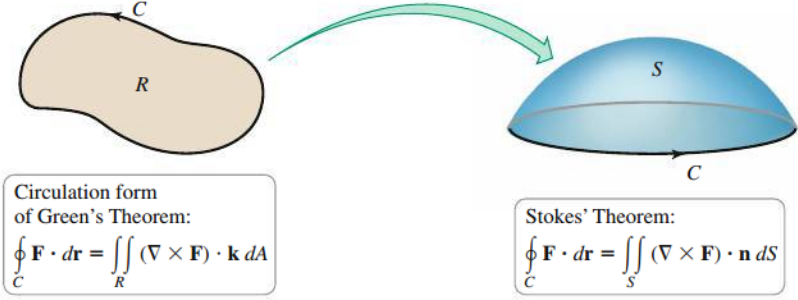
\includegraphics[width=0.75\linewidth]{images/briggs_17_07/fig17_59}
  \end{center}
  \vspace*{\stretch{1}}

  \begin{thmBox*}[Theorem 17.15: Stokes' Theorem]
    Let $S$ be an oriented surface in $\bbr^3$ with a piecewise-smooth closed boundary $C$ whose orientation is consistent with that of $S$. Assume $\mathbf F=\bracket{f,\,g,\,h}$ is a vector field whose components have continuous first partial derivatives on $S$. Then
      \[\oint\limits_C \mathbf F\cdot d\vecr=\iint\limits_S \parens{\grad\times\mathbf F}\cdot\vecn\,dS,\]
    where $\vecn$ is the unit vector normal to $S$ determined by the orientation of $S$.
  \end{thmBox*}
  \pagebreak

  \begin{ex*}
    \textbf{Verify Stokes' Theorem:} Confirm that Stokes' Theorem holds for the vector field $\mathbf F=\bracket{z-y,\,x,\,-x}$, where $S$ is the hemisphere $x^2+y^2+z^2=4$, for $z\geq 0$, and $C$ is the circle $x^2+y^2=4$, oriented counterclockwise.
  \end{ex*}
  \vspace*{\stretch{1}}
  \pagebreak

  \begin{ex*}
    Evaluate the line integral $\oint_C \mathbf F\cdot d\vecr$, where $\mathbf F=\bracket{z,\,-z,\, x^2-y^2}$ and $C$ consists of the three line segments that bound the plane $z=8-4x-2y$ in the first octant.
  \end{ex*}
  \begin{flushright}
    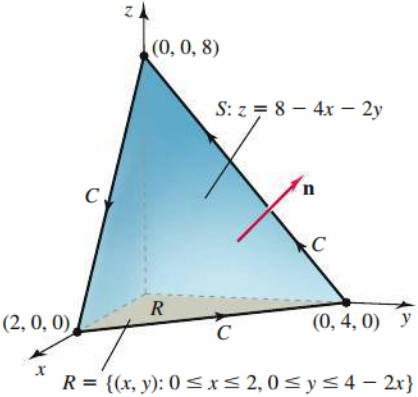
\includegraphics[width=0.35\linewidth]{images/briggs_17_07/fig17_62}
  \end{flushright}
  \vspace*{\stretch{1}}
  \pagebreak

  \begin{ex*}
    Evaluate $\iint_S \parens{\grad\times\mathbf F}\cdot\vecn\,dS$, where $\mathbf F=\bracket{-y,\,x,\,z}$, where:
  \end{ex*}

  \noindent
  \begin{minipage}[t]{0.55\linewidth}
    \begin{tasks}[after-item-skip=\stretch{1}, label=\textbullet, item-indent=0pt](1)
      \task $S$ is the part of the paraboloid $z=4-x^2-3y^2$ contained within $z=3x^2+y^2$, with $\vecn$ pointing upwards.
    \end{tasks}
  \end{minipage}%
  \begin{minipage}[t]{0.45\linewidth}\mbox{}
    \vspace*{-1.5\baselineskip}
    \begin{flushright}
      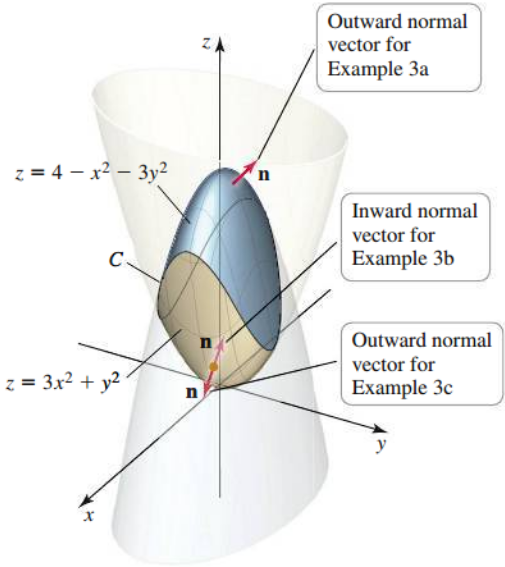
\includegraphics[width=0.78\linewidth]{images/briggs_17_07/fig17_63}
    \end{flushright}
  \end{minipage}%
  \vspace*{\stretch{1}}
  \pagebreak
  \begin{tasks}[after-item-skip=\stretch{1}, label=\textbullet, item-indent=0pt, resume](1)
    \task $S$ is the part of the paraboloid $z=3x^2+y^2$ contained within $z=4-x^2-3y^2$ with $\vecn$ pointing upwards.
  \end{tasks}
  \begin{flushright}
    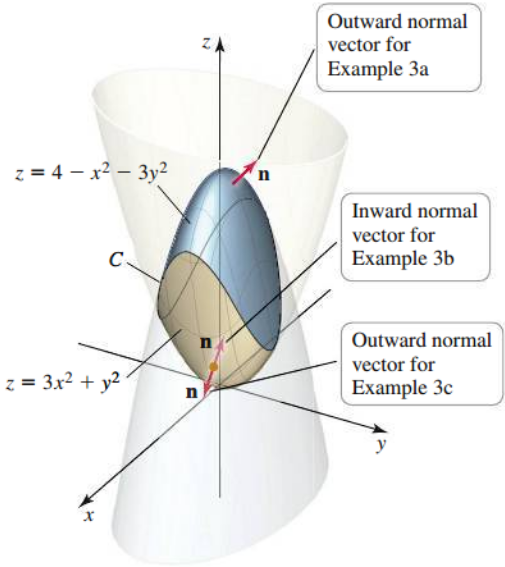
\includegraphics[width=0.35\linewidth]{images/briggs_17_07/fig17_63}
  \end{flushright}
  \vspace*{\stretch{0.75}}
  \begin{tasks}[after-item-skip=\stretch{1}, label=\textbullet, item-indent=0pt, resume](1)
    \task $S$ is the part of the paraboloid $z=3x^2+y^2$ contained within $z=4-x^2-3y^2$ with $\vecn$ pointing downwards.
  \end{tasks}
  \vspace*{\stretch{1}}
  \pagebreak

  \textbf{Interpreting the Curl:}

  The \textbf{average circulation} is 
    \[\frac{1}{\textnormal{area of }S}\oint\limits_C \mathbf F\cdot d\vecr=\frac{1}{\textnormal{area of }S}\iint\limits_S \parens{\grad\times\mathbf F}\cdot\vecn\,dS.\]

  Consider a general rotation field $\mathbf F=\veca\times\vecr$, where $\veca=\bracket{a_1,\,a_2,\,a_3}$ and $\vecr=\bracket{x,\,y,\,z}$. Now, let $S$ be a small circular disk centered at a point $P$, whose normal vector $\vecn$ makes an angle $\theta$ with the axis $\veca$:
  \begin{center}
    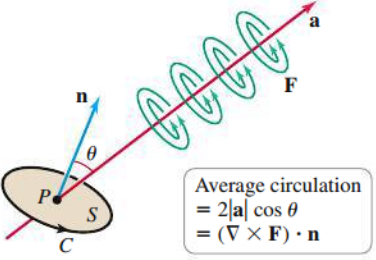
\includegraphics[width=0.4\linewidth]{images/briggs_17_07/fig17_64}
  \end{center}
  \vspace*{\stretch{1}}
  The average circulation of this vector field on $S$ is
  \begin{align*}
    \frac{1}{\textnormal{area of }S} \iint\limits_S \parens{\grad\times\mathbf F}\cdot\vecn\,dS
      &=\frac{\parens{\grad\times\mathbf F}\cdot\vecn}{\textnormal{area of }S} \,\parens{\textnormal{area of }S}\\
      &=2\veca\cdot\vecn\\
      &=2\abs{\veca}\cos(\theta)
  \end{align*}
  From this, we see
  \begin{itemize}
    \item The scalar component of $\grad\times\mathbf F$ at $P$ in the direction of $\vecn$ is the average circulation of $\mathbf F$ on $S$.
    \item The direction of $\grad\times\mathbf F$ at $P$ is the direction that maximizes the average circulation of $\mathbf F$ on $S$.
  \end{itemize}
  A similar argument for the curl can be applied to more general vector fields.
  \pagebreak

  \begin{ex*}
    Consider the vector field $\vecv=\bracket{0,\,1-x^2,\,0}$ for $\abs{x}\leq 1$ and $\abs{z}\leq 1$. Compute the curl of $\vecv$.
  \end{ex*}
  \vspace*{\stretch{1}}
  \begin{center}
    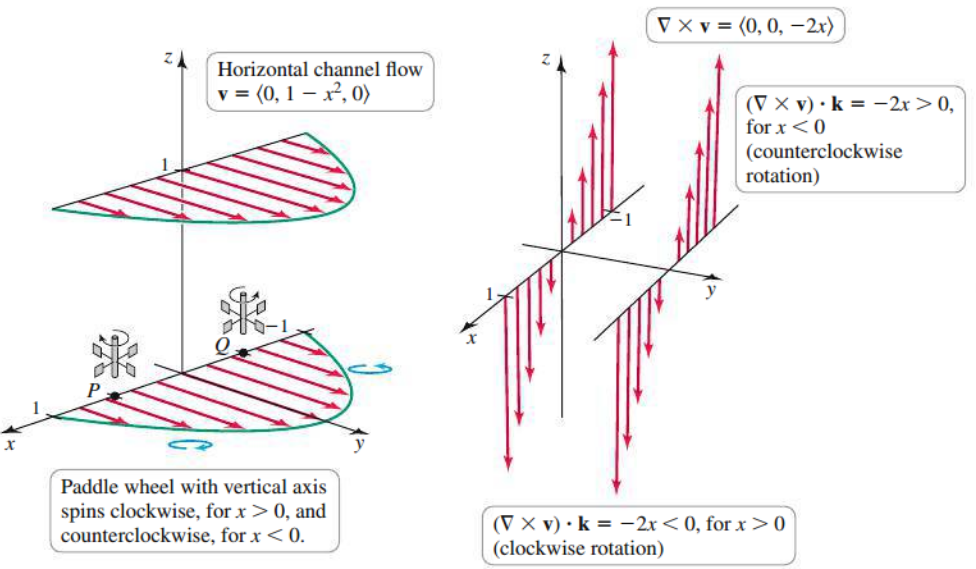
\includegraphics[width=0.75\linewidth]{images/briggs_17_07/fig17_65}
  \end{center}
  \pagebreak

  \noindent
  Since, using Stokes' Theorem, we evaluate the surface integral $\iint_S \parens{\grad\times\mathbf F}\cdot\vecn\,dS$ using only the boundary $C$, then for any two smooth oriented surfaces $S_1$ and $S_2$ both with a consistent orientation with that of $C$,
    \[\iint\limits_{S_1}\parens{\grad\times\mathbf F}\cdot\vecn_1\,dS=\iint\limits_{S_2}\parens{\grad\times\mathbf F}\cdot\vecn_2\,dS\]
  \begin{center}
    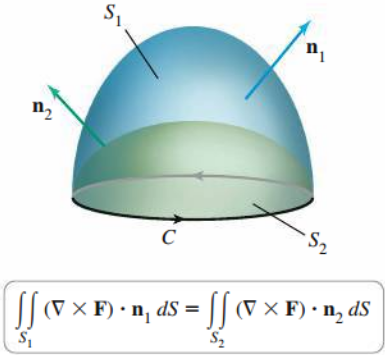
\includegraphics[width=0.27\linewidth]{images/briggs_17_07/fig17_67a}
    \hspace*{10pt}
  \end{center}

  \noindent
  Furthermore, if $S$ is a closed surface consisting of $S_1$ and $S_2$, with $\vecn=\vecn_1$ and $\vecn=-n_2$, then 
    \[\iint\limits_S \parens{\grad\times\mathbf F}\cdot\vecn\,dS=\iint\limits_{S_1}\parens{\grad\times\mathbf F}\cdot\vecn\,dS+\iint\limits_{S_2}\parens{\grad\times\mathbf F}\cdot\vecn\,dS=0\]
  \begin{center}
    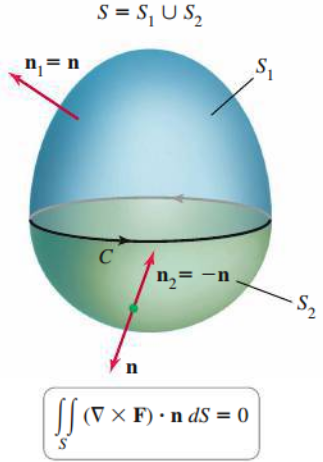
\includegraphics[width=0.27\linewidth]{images/briggs_17_07/fig17_67b}
  \end{center}
  \pagebreak

  \noindent
  Theorem 17.11 (Section 17.5) states that if $\mathbf F$ is conservative, then $\grad\times\mathbf F=\bfO$. Now, the converse follows using Stokes' Theorem:

  \begin{thmBox*}[Theorem 17.16: Curl $\mathbf F=\bfO$ implies $\mathbf F$ Is Conservative]
    Suppose $\grad\times\mathbf F=\bfO$ throughout an open simply connected region $D$ of $\bbr^3$. Then $\oint_C\mathbf F\cdot d\vecr=0$ on all closed simple smooth curves $C$ in $D$, and $\mathbf F$ is a conservative vector field on $D$.
  \end{thmBox*}
  \begin{proof}
    Given a closed simple smooth curve $C$, it can be shown that $C$ is the boundary of at least one smooth oriented surface $S$ in $D$. By Stokes' Theorem,
      \[\oint\limits_C \mathbf F\cdot d\vecr=\iint\limits_S \underbrace{\parens{\grad\times\mathbf F}}_{0}\cdot\vecn\,dS=0\]
    Since the line integral equals zero over all such curves in $D$, the vector field is conservative on $D$.
  \end{proof}

  \pagebreak
  
\end{document}